\documentclass[../psets.tex]{subfiles}

\pagestyle{main}
\renewcommand{\leftmark}{Problem Set 4}

\begin{document}




\begin{enumerate}[label={\Roman*)}]
    \item \marginnote{2/15:}In our description for a one-dimensional $s$-orbital chain with period $a$, the allowed energy states broaden into a band whose dispersion (dependence of the energy $E$ on the wavevector $k$) is given by
    \begin{equation*}
        E(k) = \alpha+2\beta\cos ka
    \end{equation*}
    where $\beta$ is the nearest-neighbor interaction energy and is less than zero for neighboring $s$-type orbitals.
    \begin{enumerate}[label={\alph*.}]
        \item Sketch $E(k)$ over the range $-\frac{\pi}{a}<k<\frac{\pi}{a}$, assuming that $\beta<0$.
        \begin{proof}[Answer]
            ${\color{white}hi}$
            \begin{center}
                \begin{tikzpicture}
                    \footnotesize
                    \draw (4,0) node[below]{$\pi/a$} -- (0,0) node[below=5mm]{\small$k\longrightarrow$} node[below]{$0$} -- (-4,0) node[below]{$-\pi/a$};
                    \draw (0,0) -- node[left=2mm,align=center]{\small$\uparrow$\\$E$} (0,3.3);
                    \draw (0.1,0.5) -- ++(-0.2,0) node[below left]{$\alpha+2\beta$};
                    \draw (0.1,2.9) -- ++(-0.2,0) node[left]{$\alpha-2\beta$};
        
                    \draw [grx,thick] (-4,2.9) cos (-2,1.7) sin (0,0.5) cos (2,1.7) node[above left,black]{\small$E(k)$} sin (4,2.9);
                \end{tikzpicture}
            \end{center}
        \end{proof}
        \item Suppose there is one electron for every 4 atoms; that is, if there are $N$ atoms in the chain, there are $N/4$ electrons. With $a=\SI{2.00e-10}{\meter}$ (i.e., $\SI{2.00}{\angstrom}$) and $\beta=\SI{-2.00}{eV}$, calculate the value of $k$ corresponding to the highest occupied electronic state (also known as Fermi wavevector $k_F$, the wavevector at the Fermi surface) and the height of the Fermi energy $E_F$ above the bottom of the band. Note that a chain of $N$ atoms will have a total length $L=Na$ and that states are uniformly distributed in the $k$-space.
        \begin{proof}[Answer]
            \begin{figure}[H]
                \centering
                \begin{subfigure}[b]{0.7\linewidth}
                    \centering
                    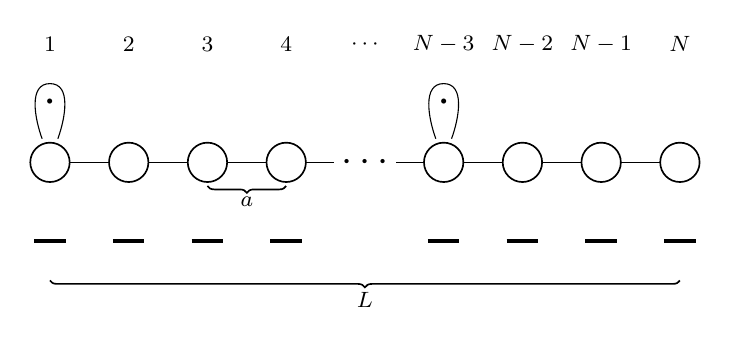
\begin{tikzpicture}
                        \footnotesize
                        \draw (0,0) -- (8,0);
                        \foreach \x in {0,1,2,3,5,6,7,8} {
                            \filldraw [semithick,fill=white] (\x,0) circle (2.5mm);
                        }
                        \node [fill=white] at (4,0) {\Large$\cdots$};
                        \foreach \x in {0,5} {
                            \draw ({\x-0.1},0.3)
                                to[out=110,in=180] (\x,1) node[below]{\LARGE$\cdot$}
                                to[out=0,in=70] ({\x+0.1},0.3)
                            ;
                        }
            
                        \foreach \x in {1,2,3} {
                            \node at ({\x-1},1.5) {$\x$};
                            \node at ({8-\x},1.5) {$N-\x$};
                        }
                        \node at (3,1.5) {$4$};
                        \node at (8,1.5) {$N$};
                        \node at (4,1.5) {$\cdots$};
            
                        \foreach \x in {1,2,3,6,7,8} {
                            \draw [ultra thick] ({\x-0.2},-1) -- ++(0.4,0);
                        }
                        \foreach \x in {0,5} {
                            \draw [ultra thick] ({\x-0.2},-1) -- node{\Large$\upharpoonleft$} ++(0.4,0);
                        }
            
                        \draw [semithick,decorate,decoration={brace,mirror}] (2,-0.3) -- node[below=1pt]{$a$} ++(1,0);
                        \draw [semithick,decorate,decoration={brace,mirror}] (0,-1.5) -- node[below=1pt]{$L$} ++(8,0);
                    \end{tikzpicture}
                    \caption{The orbital chain and its states.}
                    \label{fig:s-orbitalsa}
                \end{subfigure}\\[1em]
                \begin{subfigure}[b]{0.8\linewidth}
                    \centering
                    \begin{tikzpicture}[
                        xscale=0.8,
                        every node/.append style={black}
                    ]
                        \footnotesize
                        \fill [grz] (-2,-0.07) rectangle (2,0.07);
            
                        \draw (-8,0) -- (8,0);
                        \draw (-8,0.1) -- ++(0,-0.2) node[below]{$-\pi/a$};
                        \draw (8,0.1) -- ++(0,-0.2) node[below]{$\pi/a$};
                        \draw (-2,0.1) -- ++(0,-0.2) node[below]{$-k_F$};
                        \draw (2,0.1) -- ++(0,-0.2) node[below]{$k_F$};
            
                        \draw (0,4) -- (0,-0.1) node[below]{$0$};
                        \draw (0.1,0.5) -- ++(-0.2,0) node[below left]{$\alpha+2\beta$};
                        \draw (0.1,3.5) -- ++(-0.2,0) node[left]{$\alpha-2\beta$};
            
            
                        \foreach \x in {-8,...,8} {
                            \fill (\x,0) circle (1pt);
                        }
            
                        \draw [grx,thick] (-8,3.5) cos (-4,2) sin (0,0.5) node[below right]{$E(0)$} cos (4,2) sin (8,3.5);
                        \draw [grx,dashed] (-2,0) -- (-2,0.939) -- node[above right]{$E(k_F)$} (2,0.939) -- (2,0);
            
                        \draw [decorate,decoration={brace,mirror}] (-2,-0.7) -- node[below=1pt]{$2k_F$} (2,-0.7);
                    \end{tikzpicture}
                    \caption{$k$-space and energy.}
                    \label{fig:s-orbitalsb}
                \end{subfigure}
                \caption{Theory describing a one-dimensional $s$-orbital chain.}
                \label{fig:s-orbitals}
            \end{figure}
            As in Figure \ref{fig:s-orbitalsa}, consider a one-dimensional chain of $N$ atoms with one $s$-orbital each. The orbitals are separated by period $a$, and the length of the chain is $L=Na$. As in Figure \ref{fig:s-orbitalsb}, each orbital contributes a state indexed by $k$. These states are evenly distributed in one-dimensional $k$-space between $-\frac{\pi}{a}$ and $\frac{\pi}{a}$. Now imagine that the one-dimensional $s$-orbital chain is devoid of electrons, and we have to fill them in. The first electron will go in the lowest energy state at $k=0$ (see Figure \ref{fig:s-orbitalsb}). The second will go into either $k=a$ or $k=-a$, and the third will go into the other one. As we add more and more electrons, the states that they go into will expand outwards evenly from the origin, always filling the lowest energy states available first. Eventually, all electrons will be filled in; however, this does not mean that all states will be filled, as there is one electron for every four atoms and, thus, for every eight states (again, see Figure \ref{fig:s-orbitalsa}). Indeed, some region evenly surrounding the origin will be completely filled in, and by definition the Fermi surface will be the boundary between occupied and unoccupied states. Since the Fermi wavevector $k_F$ is the radius of the Fermi surface (i.e., the distance from the origin to the boundary of the Fermi sphere), we can label the boundary points $k_F$ and $-k_F$. Having established the theoretical design, let's start the actual calculations.\par
            Since $k$-space within the first Brillouin zone runs from $-\frac{\pi}{a}$ to $\frac{\pi}{a}$, the length of the $s$-orbital chain in $k$-space is $L=\frac{\pi}{a}-(-\frac{\pi}{a})=\frac{2\pi}{a}$. It follows that each orbital is separated by $a=\frac{2\pi}{L}$, and that there are $\frac{L}{2\pi}$ orbitals per unit length. Now the length of the occupied region is $k_F-(-k_F)=2k_F$, so combining this with the previous result gives us that there are $2k_F\times\frac{L}{2\pi}=\frac{k_FL}{\pi}$ occupied orbitals. Since each orbital adds 2 quantum states, we have $\frac{2k_FL}{\pi}$ occupied states. But the number of occupied states is simply equal to the number of electrons $\frac{N}{4}$. Since we also know that $L=Na$, we have that
            \begin{align*}
                \frac{2k_FNa}{\pi} &= \frac{N}{4}\\
                \frac{k_Fa}{\pi} &= \frac{1}{8}\\
                k_F &= \frac{\pi}{8a}\\
                \Aboxed{k_F &= \SI{1.96e9}{\per\meter}}
            \end{align*}
            As to the other part of the question, refer to Figure \ref{fig:s-orbitalsb} once again. It tells us that the height of the Fermi energy above the bottom of the band is given by
            \begin{align*}
                h &= E(k_F)-E(0)\\
                &= \alpha+2\beta\cos\left( \frac{\pi}{8a}\cdot a \right)-(\alpha+2\beta\cos(0\cdot a))\\
                &= 2\beta\left( \cos\left( \frac{\pi}{8} \right)-1 \right)\\
                \Aboxed{h &= \SI{0.304}{eV}}
            \end{align*}
        \end{proof}
    \end{enumerate}
    \newpage
    \item Do the following problems from Chapter 6: 13, 25, 30, 37.
    \begin{enumerate}[label={\textbf{6.\arabic*}}]
        \setcounter{enumii}{12}
        \item If an equimolar mixture of \ce{P($t$-C4H9)3} and \ce{B(C6F5)3} is mixed with $\SI{1}{\bar}$ of the gas \ce{N2O} in bromobenzene solution, a white product is formed in good yield. A variety of NMR evidence has been gathered on the product: there is a single \ce{^{31}P} NMR resonance; \ce{^{11}B} and \ce{^{19}F} NMR are considered consistent with a 4-coordinate boron atom; and \ce{^{15}N} NMR indicates two nonequivalent nitrogen atoms. In addition, no gas is released in the reaction.
        \begin{enumerate}[label={\textbf{\alph*.}}]
            \item Suggest the role of \ce{N2O} in this reaction.
            \begin{proof}[Answer]
                \ce{N2O} reorganizes into a bridge linking the phosphorous and boron central atoms of \ce{P($t$-C4H9)3} and \ce{B(C6F5)3}, respectively. \ce{P($t$-C4H9)3} contains a frustrated Lewis pair that could not normally react with the boron in \ce{B(C6F5)3}, but by virtue of this bridge, there is enough separation between all of the substituents (i.e., steric hindrance is sufficiently reduced) to permit the formation of a combined product.
            \end{proof}
            \item Propose a structure of the product.
            \begin{proof}[Answer]
                ${\color{white}hi}$
                \begin{center}
                    \chemfig{\ce{($t$-Bu)3}P-N=[:-30]N-O-[:-30]B}
                    \begin{tikzpicture}[remember picture,overlay]
                        \node at (0.5,-0.9) {\ce{(C6F5)3}};
                    \end{tikzpicture}
                \end{center}
            \end{proof}
        \end{enumerate}
        \newpage
        \setcounter{enumii}{24}
        \item The most common source of mercury is cinnabar (\ce{HgS}), whereas \ce{Zn} and \ce{Cd} in the same group occur as sulfide, carbonate, silicate, and oxide. Why?
        \begin{proof}[Answer]
            Mercury is soft, so it forms a stable product with the similarly soft sulfide ion. However, zinc and cadmium are intermediate-hard, so they can form stable products with harder anions, such as carbonate, silicate, and oxide.
        \end{proof}
        \newpage
        \setcounter{enumii}{29}
        \item \ce{CsI} is much less soluble in water than \ce{CsF}, and \ce{LiF} is much less soluble than \ce{LiI}. Why?
        \begin{proof}[Answer]
            Cesium iodide is formed from two soft ions, which grants it extra stability in comparison to soft-hard compounds such as cesium fluoride. As such, \ce{CsI} will dissolve much less in water than \ce{CsF} since it prefers to be in the molecular state rather than the ionic state.\par
            The same is true for the hard-hard compound lithium fluoride in comparison to the hard-soft compound lithium iodide.
        \end{proof}
        \newpage
        \setcounter{enumii}{36}
        \item List the following acids in order of their acid strength when reacting with \ce{NH3}: \ce{BF3}, \ce{B(CH3)3}, \ce{B(C2H5)3}, and \ce{B[C6H2(CH3)3]3}.
        \begin{proof}[Answer]
            We have
            \begin{equation*}
                \ce{BF3} > \ce{B(CH3)3} > \ce{B(C2H5)3} > \ce{B[C6H2(CH3)3]3}
            \end{equation*}
            \ce{BF3} will be the strongest Lewis acid because it is the only one out of the collection that has electron-withdrawing groups as opposed to electron donating groups. Among the three compounds with electron-donating groups, we rank as stronger acids the ones with smaller groups, both because smaller groups donate less and the reduction in steric hindrance.
        \end{proof}
    \end{enumerate}
\end{enumerate}




\end{document}